%=================================================================
\section{Introduction}\label{sec-intro}
The project will build a model that predicts the total ride duration of taxi trips
in New York City. The primary dataset is one released by the NYC Taxi and
Limousine Commission, which includes pickup time, geo-coordinates, number of
passengers, and several other variables. Accordingly, this project problem is taxi
trips duration, which is a outlier detection. There are 6 steps including data loading
and overview, data cleaning, features engineering, model selection, hyperparameters
tuning, and training and predictions.

%\todo{Narrow down to a topic; Dig a hole; Fill the hole}
%\todo{Formula for Introduction}



%\gangli{``narrow in on topic'' reminds you 
%that readers and reviewers only know that this is a AI or HTM research paper (and maybe have read the title/abstract). 
%You need to help them figure out what topic and area of research paper this is. 
%You _don't_ need to wax poetic about the topic's importance.}

%\gangli{`dig a hole'' reminds you that 
%you need to convince the reader that there's a problem with the state of the world. 
%Prior work may exist but it's either missing something important or there's a missing opportunity. 
%The reader should be drooling for a bright future just out of reach.}

%\gangli{``fill the hole'' reminds you to show the reader 
%how and why the paper they're reading will fix these problems and deliver us into a better place. 
%You don't need a whirlwind summary of the technical details, 
%but you need readers convinced (and in a good mood) to keep reading.}

%\gangli{A good paper introduction is fairly formulaic. 
%If you follow a simple set of rules, 
%you can write a very good introduction. 
%The following outline can be varied. 
%For example, 
%you can use two paragraphs instead of one, 
%or you can place more emphasis on one aspect of the intro than another. 
%But in all cases, 
%all of the points below need to be covered in an introduction, 
%and in most papers, 
%you don't need to cover anything more in an introduction.}



%\todo{The importance of the area}
%\blindtext
%\todo{Motivation}
%At a high level, 
%what is the problem area you are working in and why is it important? 
%It is important to set the larger context here. 
%Why is the problem of interest and importance to the larger community?


%\todo{The problems faced by most current methods}
%\blindtext
%\todo{What is the specific problem considered in this paper?}
%This paragraph narrows down the topic area of the paper. 
%In the first paragraph you have established general context and importance. 
%Here you establish specific context and background.

%\todo{What can be addressed by existing methods; Why those problems are challenges to existing methods?}
%\blindtext
%\todo{Contribution}
%"In this paper, we show that ...". 
%This is the key paragraph in the intro - you summarize, 
%in one paragraph, 
%what are the main contributions of your paper given the context 
%you have established in paragraphs 1 and 2. 
%What is the general approach taken? 
%Why are the specific results significant? 
%This paragraph must be really good. 


\begin{itemize}
	\item Data loading and overview
	\item Data cleaning
	\item Features engineering
	\item Model selection
	\item Hyperparameters tuning
	\item Training and predictions
\end{itemize}


%\todo{What provides the motivation of this work? What are the research issues? What is the rationale of this work? }
%\blindtext
%\todo{At a high level what are the differences in what you are doing, and what others have done? }
%Keep this at a high level, 
%you can refer to a future section where specific details and differences will be given. 
%But it is important for the reader to know at a high level, 
%what is new about this work compared to other work in the area.

%\todo{What we have done and what are the contributions.}
%\blindtext
%\todo{A roadmap for the rest of the paper}
%"The remainder of this paper is structured as follows..." 
%Give the reader a roadmap for the rest of the paper. 
%Avoid redundant phrasing, 
%"In Section 2, In section 3, ... In Section 4, ... " etc.

%\gangli{A few general tips:
%Don't spend a lot of time into the introduction 
%telling the reader about what you don't do in the paper. 
%Be clear about what you do do.
%Does each paragraph have a theme sentence that sets the stage for the entire paragraph? Are the sentences and topics in the paragraph all related to each other?}

%\gangli{Does each paragraph have a theme 
%sentence that sets the stage for the entire paragraph? 
%Are the sentences and topics in the paragraph all related to each other?}
%
%\gangli{Do all of your tenses match up in a paragraph?}

%Test citation~\cite{BL12J01}. 
%\begin{JournalOnly}
%and~\citep{BJL11J01} or~\citet{BJL11J01}.
%\end{JournalOnly}

%This is for~\cref{tbl:overall-experiments}, 
%\todo[fancyline]{Testing.}
%and this is for~\cref{sec-conclusions}.
%\todo[noline]{A note with no line back to the text.}%
%\gangli{This is comment from Gang.}
%\qwu{Response from QW}
%
%Number:
%\num{123}.
%\numlist{10;30;50;70},
%\numrange{10}{30},
%\SIlist{10;30;45}{\metre},
%and
%\SI{10}{\percent}
%
%\missingfigure[figcolor=white]{Testing figcolor}
%
%
%\begin{ConferenceOnly}
%We have \SI{10}{\hertz},
%\si{\kilogram\metre\per\second},
%the range: \SIrange{10}{100}{\hertz}.
%$\nicefrac[]{1}{2}$.
%
%\missingfigure{Make a sketch of the structure of a trebuchet.}

%\end{ConferenceOnly}


%For~\cref{eq:test},
%as shown below:
%
%\begin{equation}\label{eq:test}
%a = b \times \sqrt{ab}
%\end{equation}
%
%\blindmathpaper

\section{Data loading and overview} \label{sec-Data loading and overview}

At first, I quickly look at the first 5 lines of a dataset to understand the structure,
format, and content of the data . Then I take a overview of the type and amount
and other information of df and test data.
\begin{figure}[h]
	\centering
	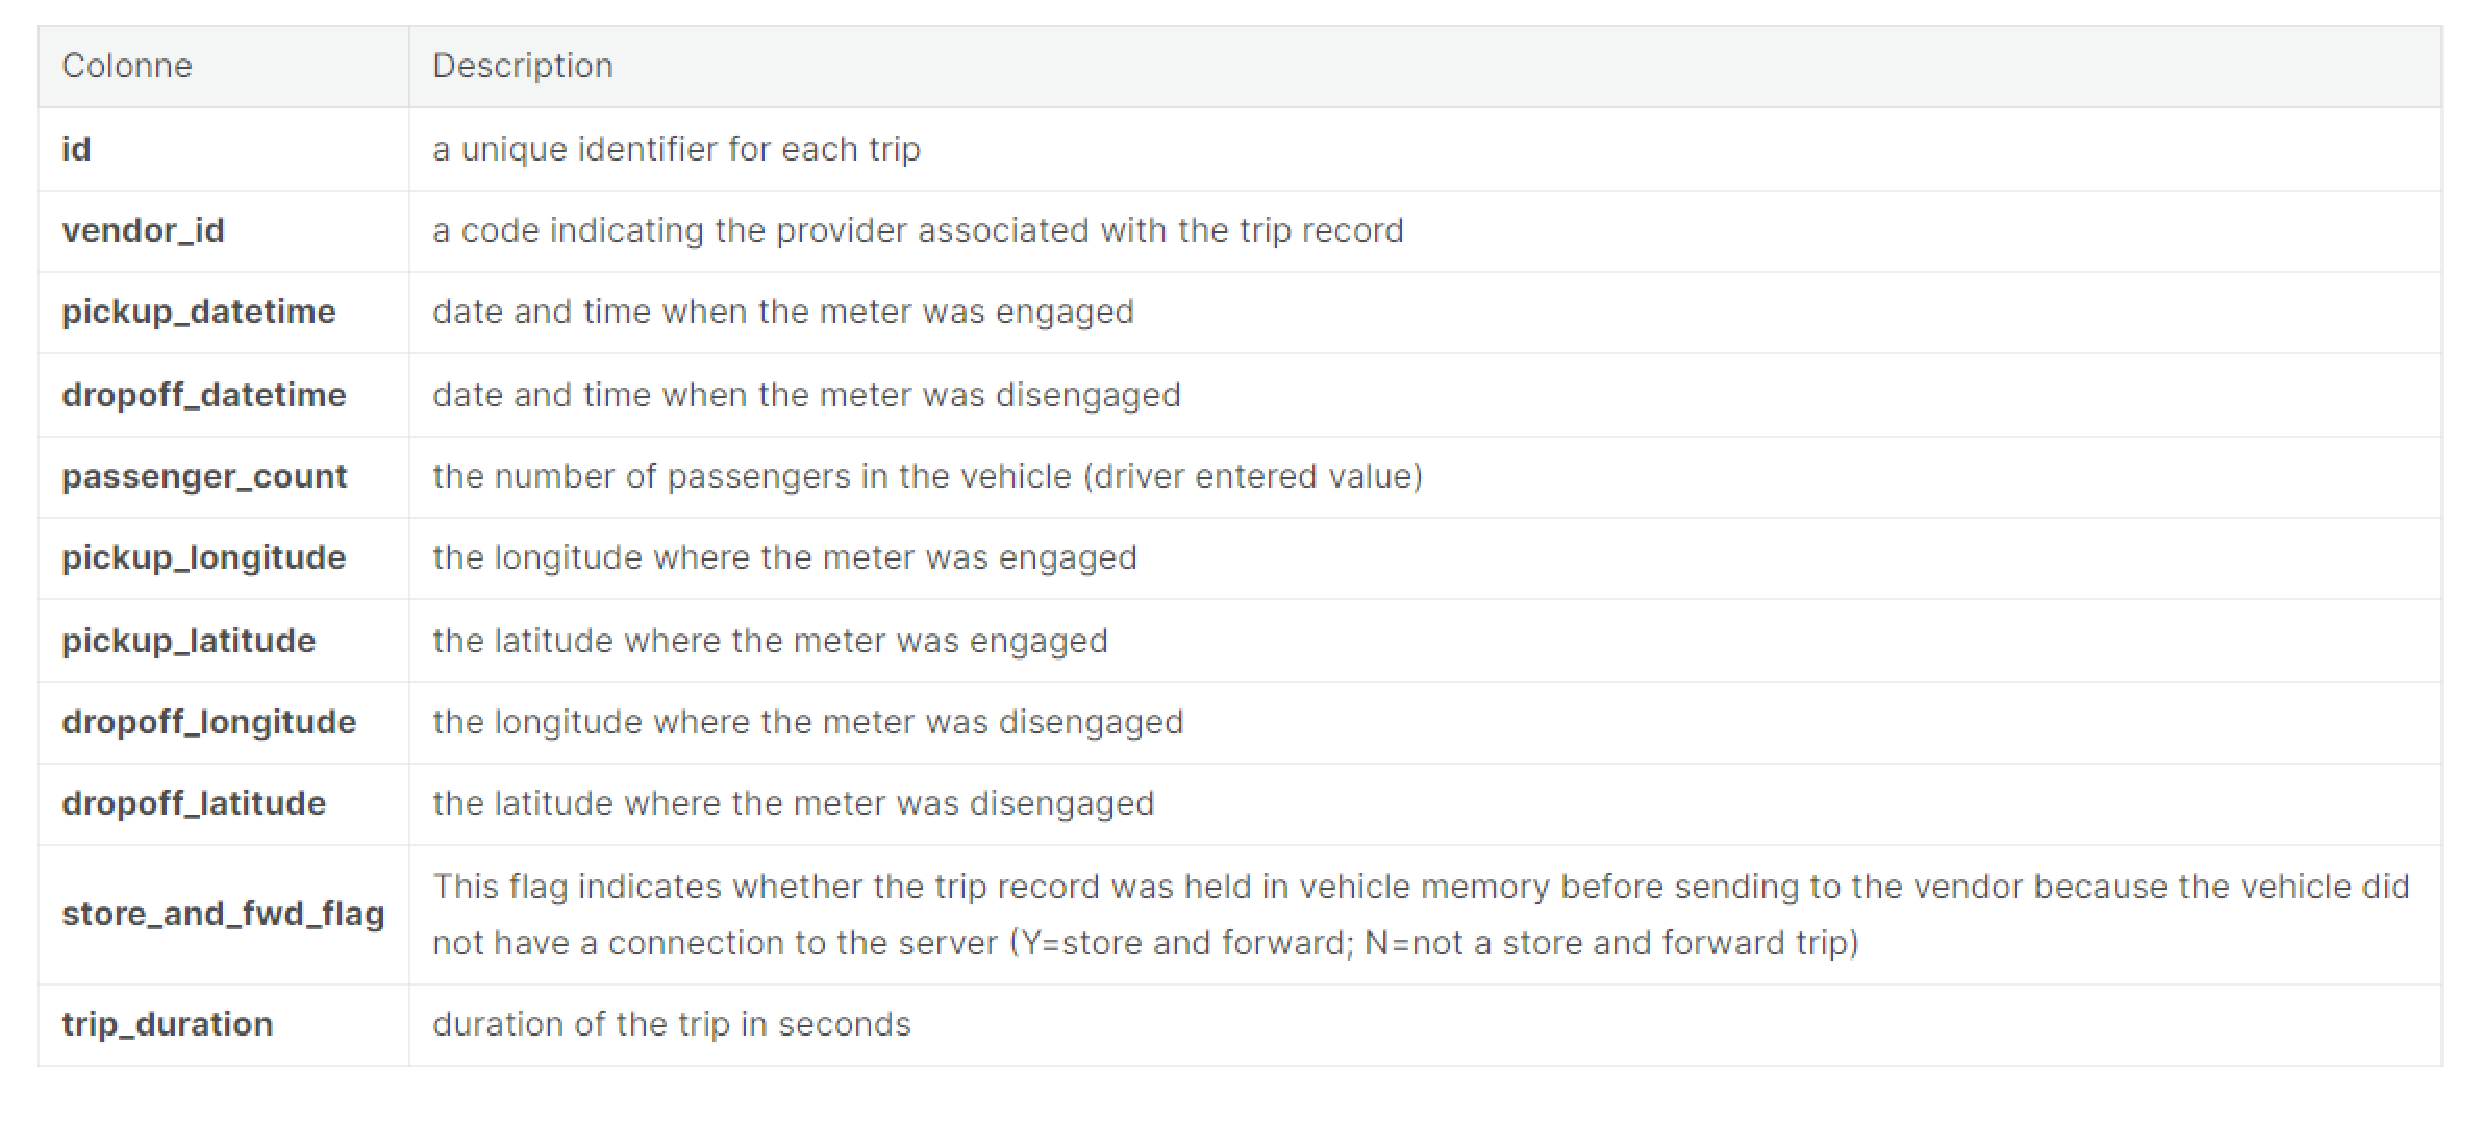
\includegraphics[scale=0.3]{overview.eps}
	\caption{overview of the data}
\end{figure}

%\gliMarker  %TODO: GLi Here

\vspace{8cm}
\section{Data cleaning} \label{sec-Data cleaning}
I do the data learning to check the duplicated and missing values and deal with outliers.
\begin{figure}[h]
	\centering
	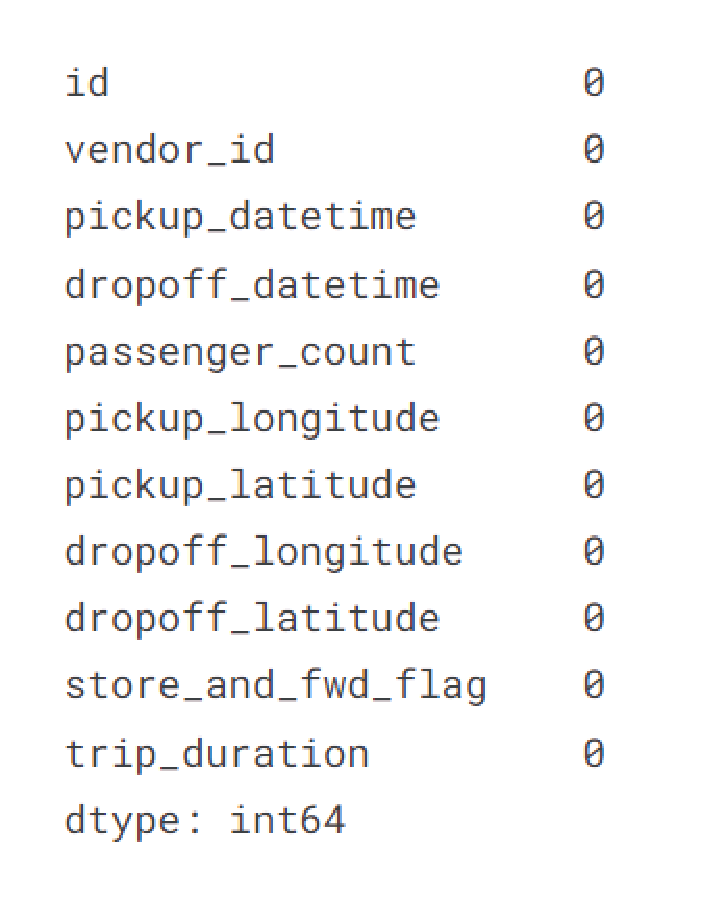
\includegraphics[scale=0.3]{duplicate.eps}
	\caption{No duplicate and missing data}
\end{figure}

\begin{itemize}
\item Visualize outliers
\end{itemize}
There are outliers. I can’t find a proper interpretation and it will probably damage our model, so I choose to get rid of them.
\begin{figure}[h]
	\centering
	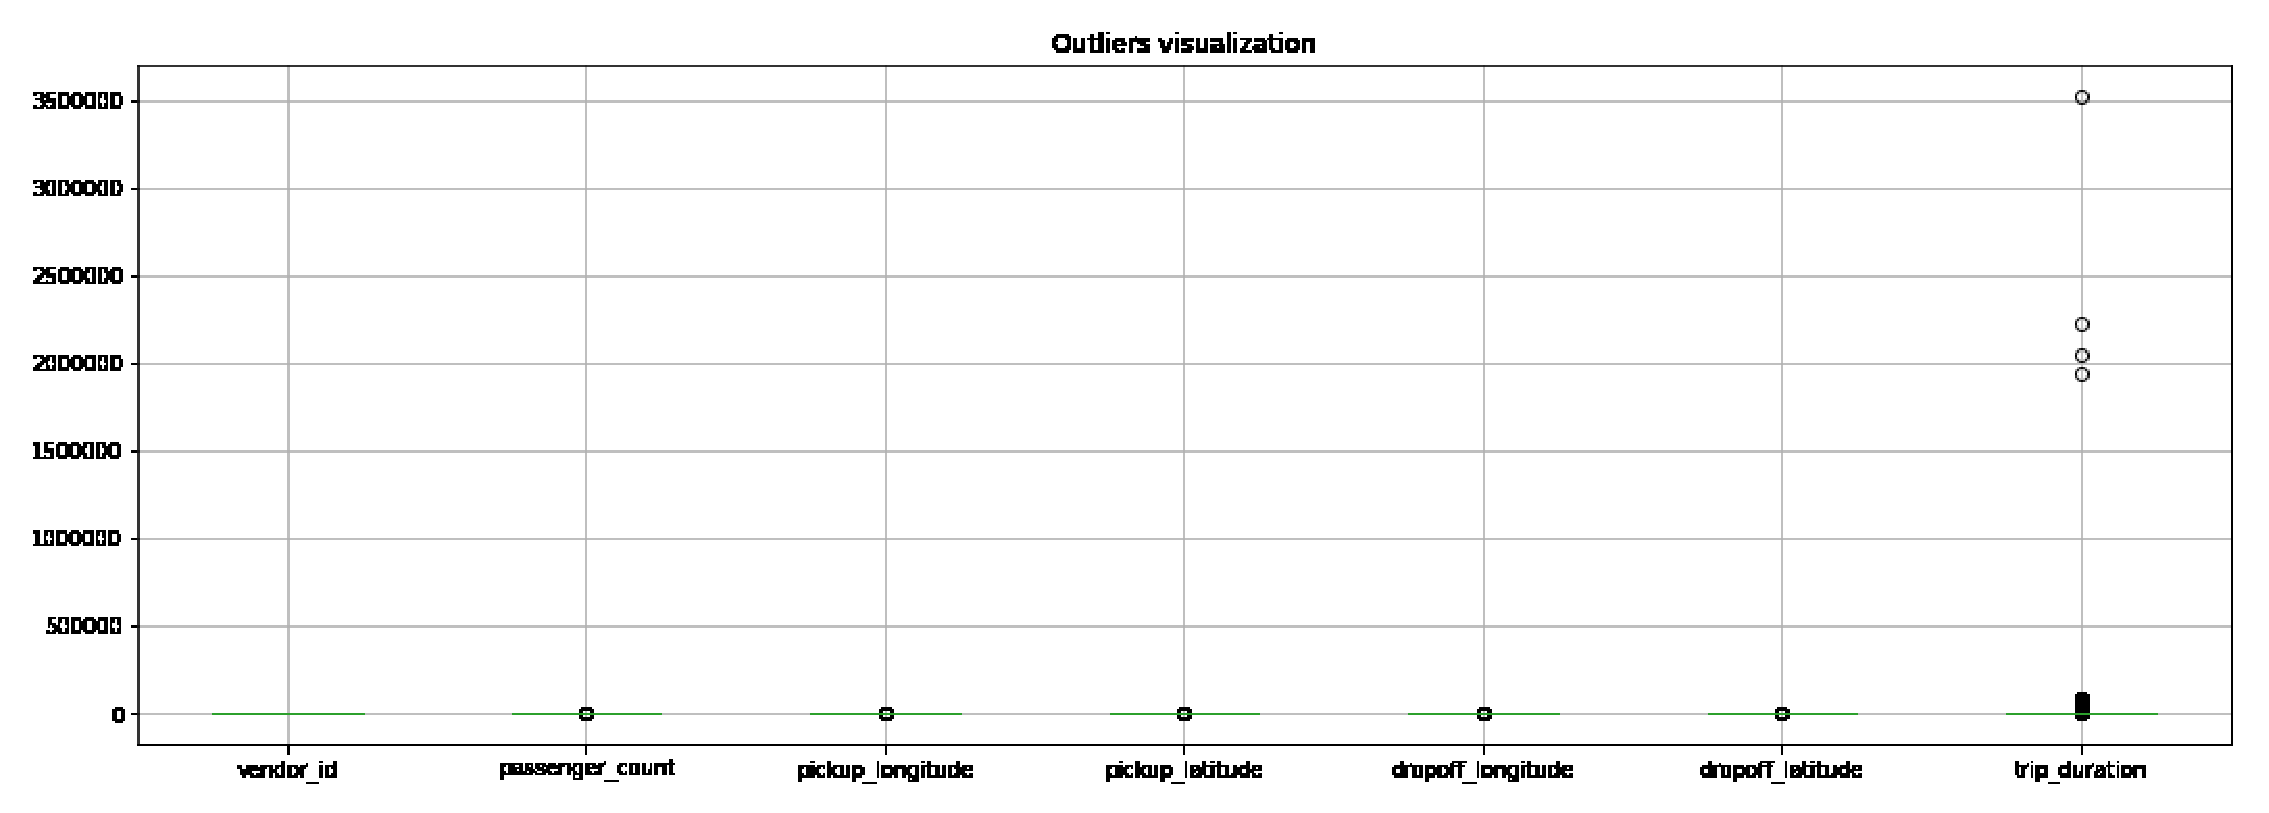
\includegraphics[scale=0.3]{outliers1.eps}
	\caption{outliers for trip-duration}
\end{figure}
\begin{figure}[h]
	\centering
	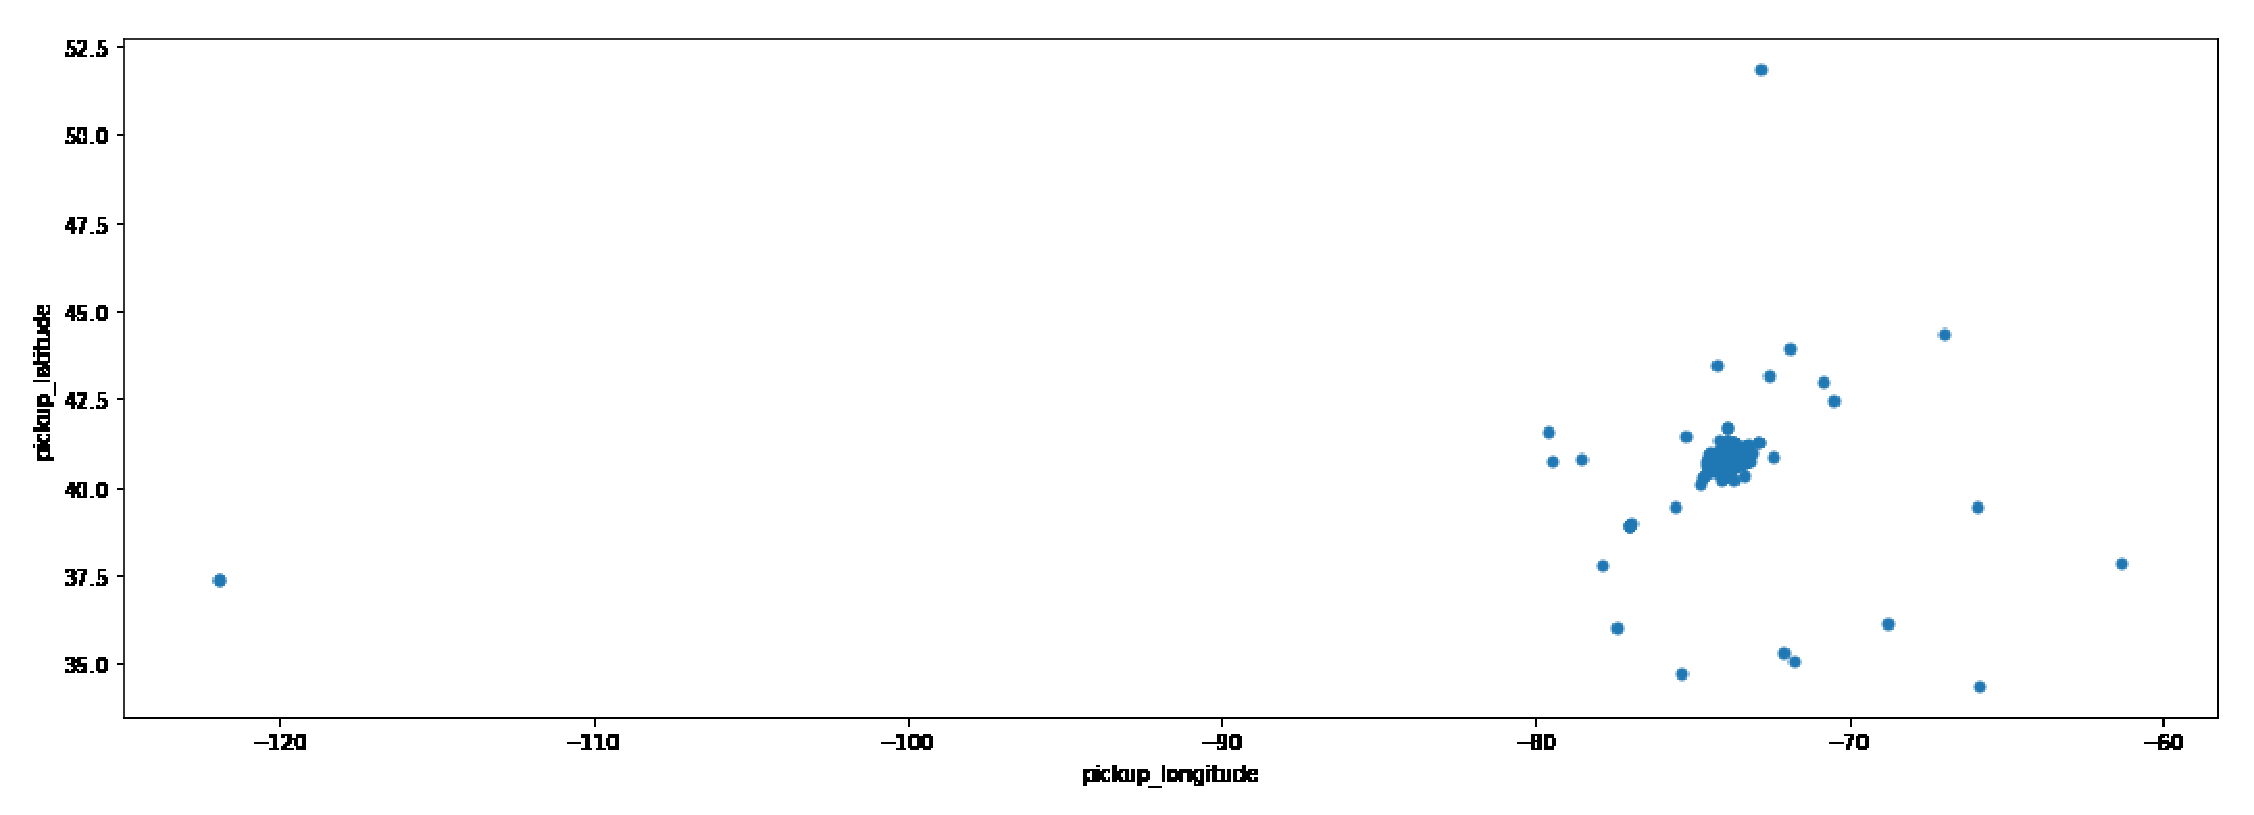
\includegraphics[scale=0.3]{outliers2.eps}
	\caption{outliers for pickup positions}
\end{figure}
\begin{figure}[h]
	\centering
	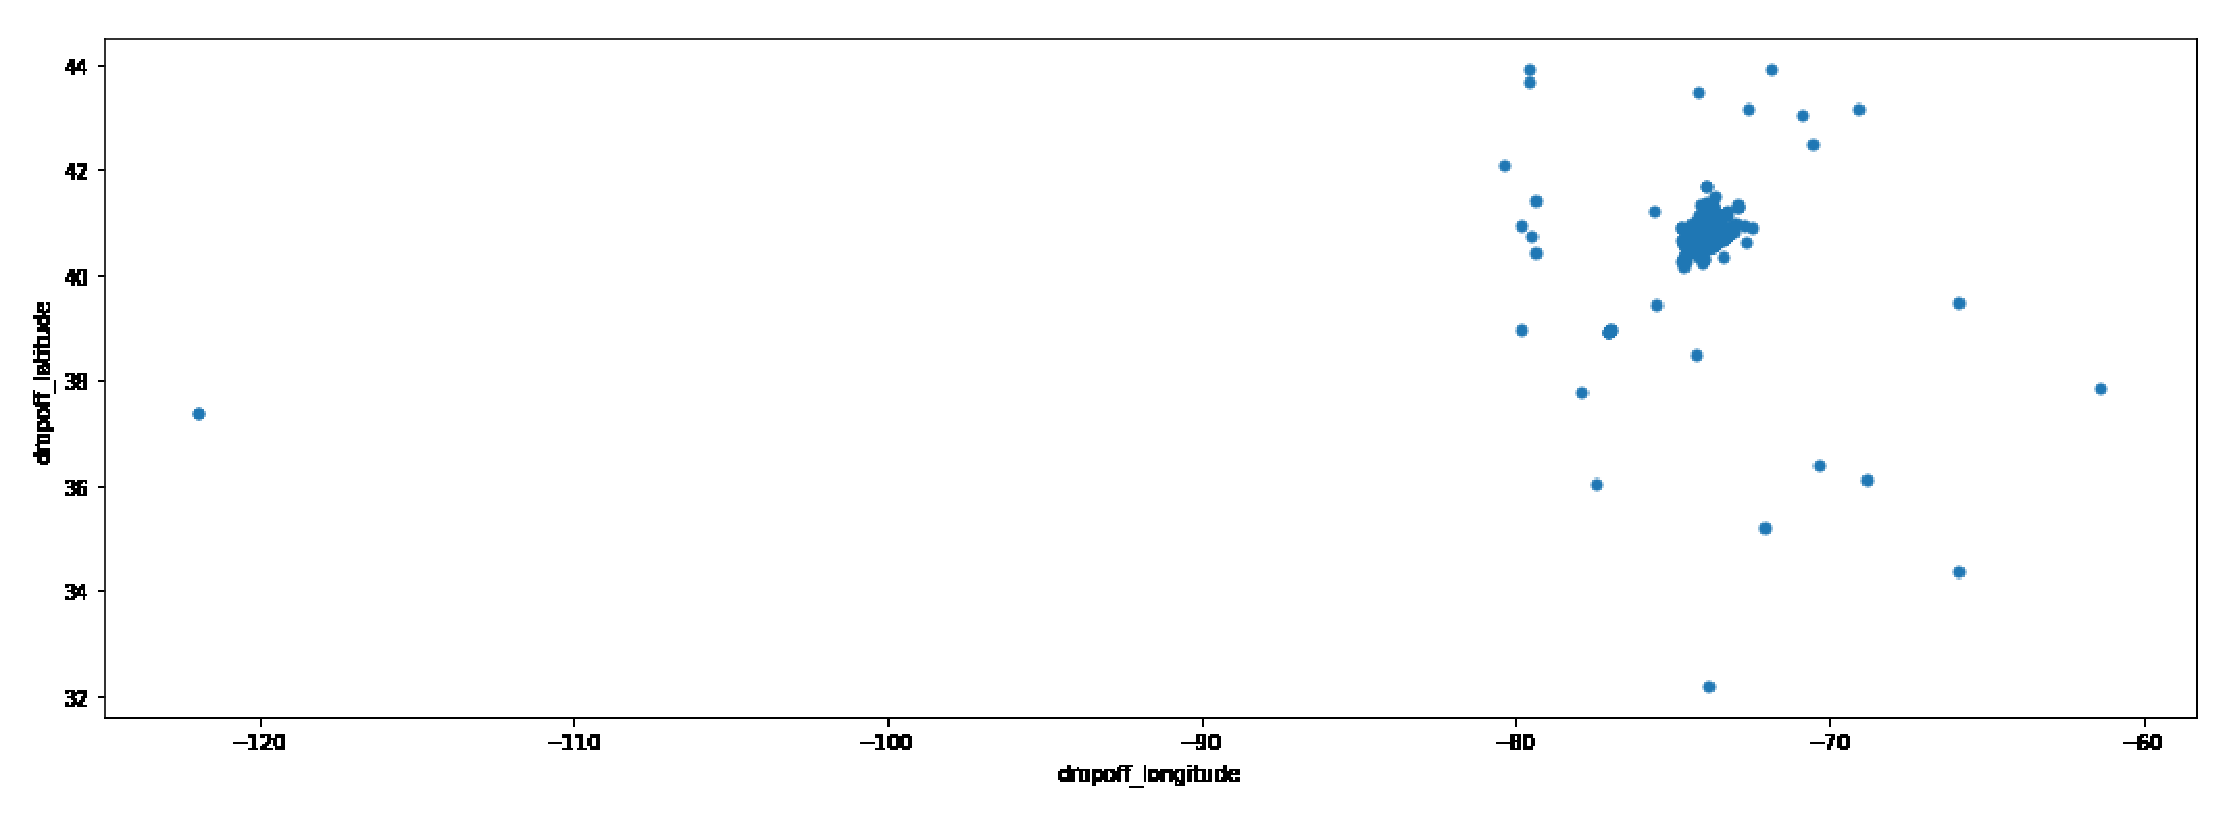
\includegraphics[scale=0.3]{outliers3.eps}
	\caption{outliers for  dropoff positions}
\end{figure}
\vspace{5cm}\\
In this step, I only keep trips that lasted less than 5900 seconds, and only keep trips with passengers.
%\blindtext
%\blindlist{itemize}[3]
%\blinditemize
%\blindenumerate
%
%\blindmathtrue
%\blindmathfalse
%\blinddescription
%
%\qwuMarker %TODO: QWu Here



\section{Features engineering} \label{sec-Features engineering}


%\begin{table}  \centering
%  \caption{Precision Comparison on Event Detection Methods}
%  \label{tbl:overall-experiments}
%  \begin{tabular}{cccc}
%\toprule
%    % after \\: \hline or \cline{col1-col2} \cline{col3-col4} ...
%    & OR Event Detection & AC Event Detection & TC Event Detection \\
%\midrule
%    precision & 0.83 & 0.69 & 0.46 \\
%    recall & 0.68 & 0.48 & 0.36 \\
%    F-score & 0.747 & 0.57 & 0.4 \\
%\bottomrule
%\end{tabular}
%\end{table}
At first, I visualize the distribution of trip-duration values.
\begin{figure}[h]
	\centering
	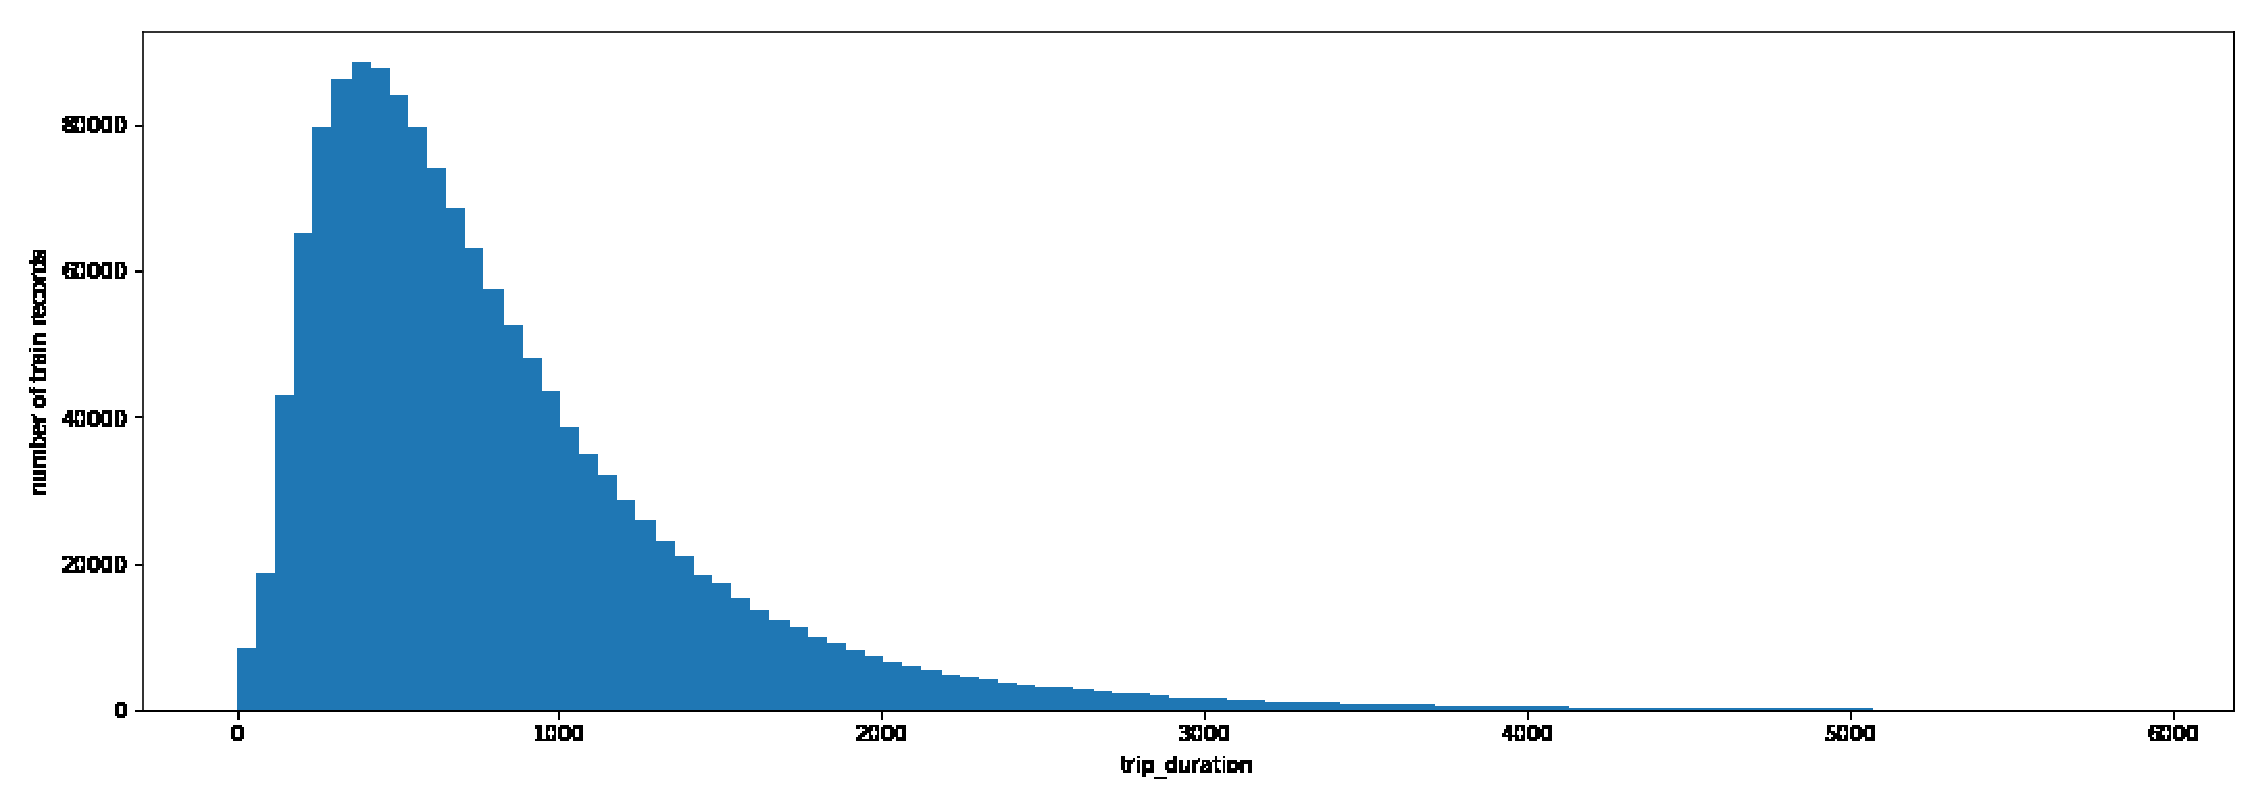
\includegraphics[scale=0.3]{trip_duration.eps}
	\caption{the distribution of trip-duration values}
\end{figure}
\\
The distribution is right-skewed so we can consider a log-transformation of trip-duration column.
\begin{figure}[h]
	\centering
	\includegraphics[scale=0.3]{log(trip_duration).eps}
	\caption{log of trip-duration}
\end{figure}
\\
Then I deal with categorical features using One-hot encoding binary categorical features.  
\\
Then I deal with dates, and ccreat distance and speed. Finally, I remove the outliers. Then we test the correlations between variables and made a figure.
\begin{figure}[h]
	\centering
	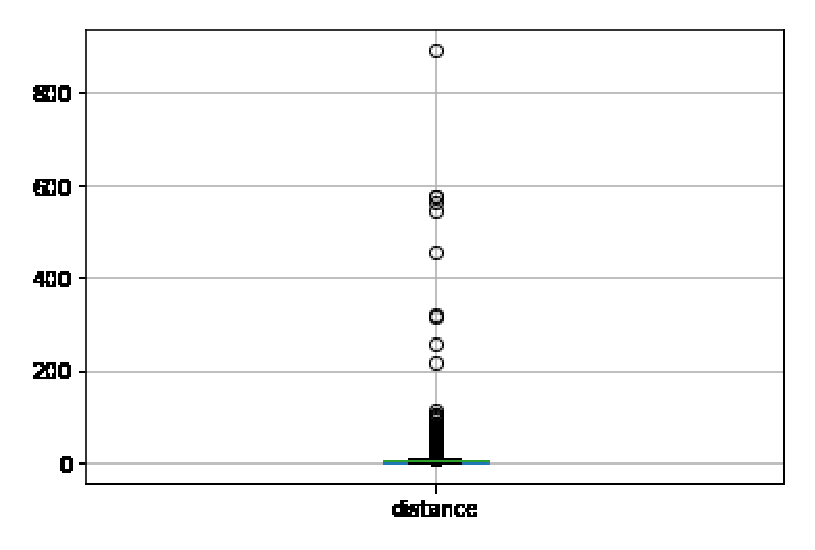
\includegraphics[scale=0.3]{distance.eps}
	\caption{outliesrs of distance}
\end{figure}
\begin{figure}[h]
	\centering
	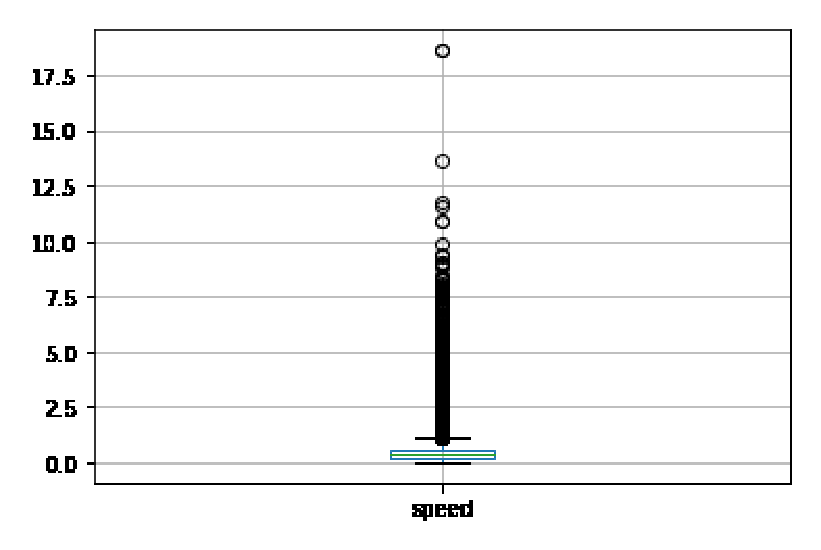
\includegraphics[scale=0.3]{speed.eps}
	\caption{outliesrs of speed}
\end{figure}
\begin{figure}[h]
	\centering
	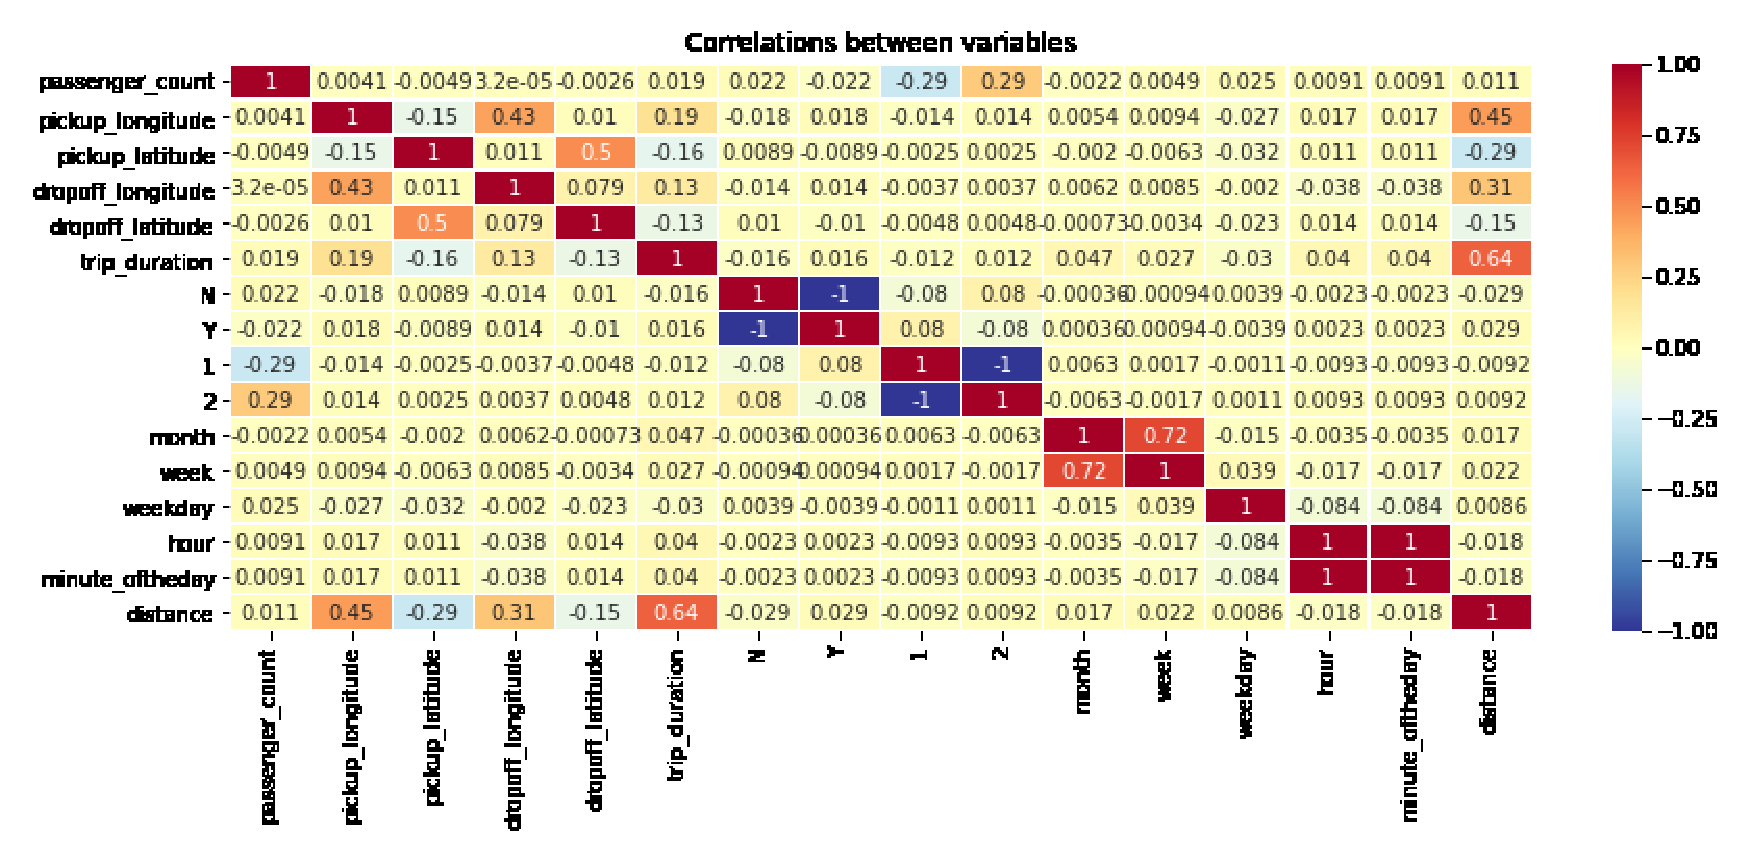
\includegraphics[scale=0.3]{correlations between variables.eps}
	\caption{correlations between variables}
\end{figure}

\section{Model selection} \label{sec-Model selection}

In this part, we split the labeled data frame into two sets: features and target to train, and then test the models. Then, for this specific problematic, we'll measure the error using the RMSE(Root Mean Squared Error). We tried GradientBoosting, RandomForest, and LightGBM. LightGBM is blazingly fast compared to RandomForest and classic GradientBoosting, while fitting better.It is our clear winner. Then we did cross-validation. The result shows that our LightGBM model is stable.

\section{Hyperparameters tuning} \label{sec-Hyperparameters tuning}
We did hyperparameters tunning using RandomizedSearchCV, and Test the following parameters:'learning-rate', 'max-depth', 'num-leaves','objective':'regression', 'feature-fraction', 'bagging-fraction', 'max-bin'.
\section{Training and predictions}
We trained on all labeled data using the best parameters in hyperparameters tuning, and trained on all labeled data using the best parameters (sklearn API version), and trained on all labeled data using the best parameters. Then we make predictions on test data frame, create a data frame designed a submission on Kaggle.
Lastly, create a csv out of the submission data frame.
\begin{figure}[h]
	\centering
	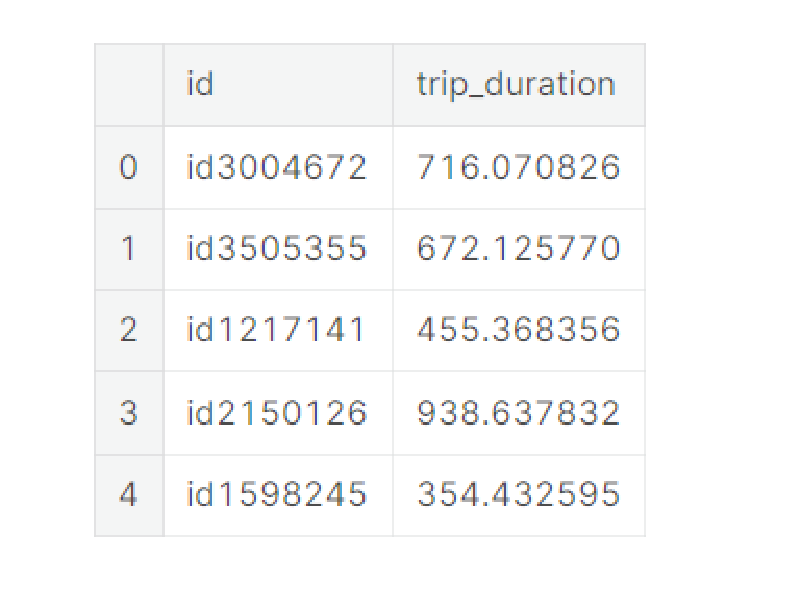
\includegraphics[scale=0.3]{predict_result.eps}
	\caption{predict-result}
\end{figure}
%\lipsum[1]


%The authors would like to thank \ldots

